\documentclass{standalone}
\usepackage{tikz}
\usetikzlibrary{patterns, positioning}


\begin{document}
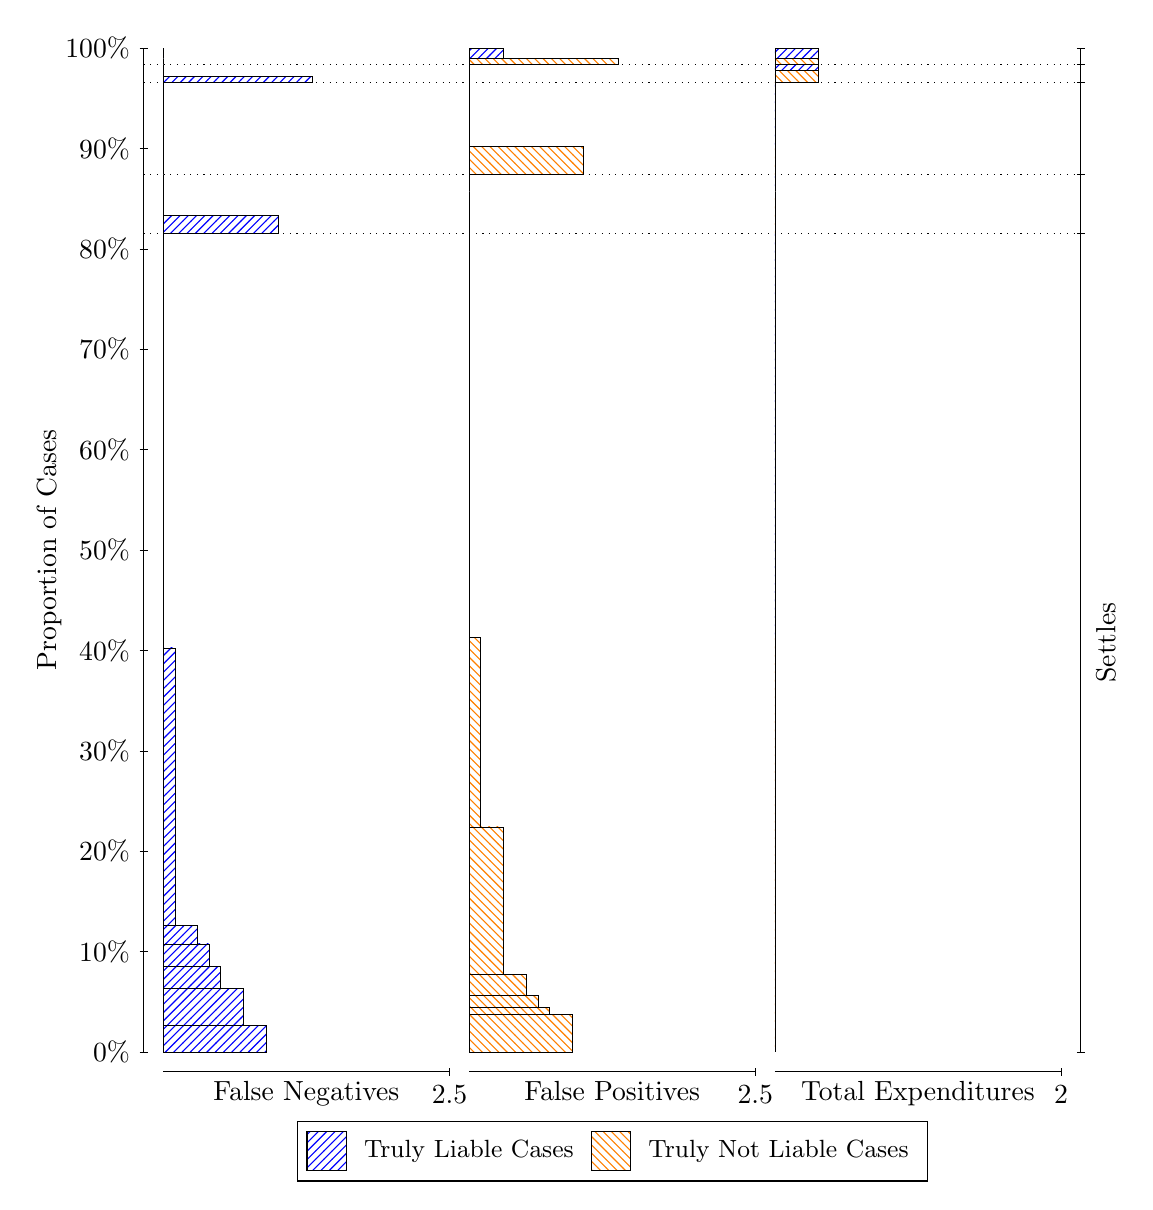
\begin{tikzpicture}
\draw[black, very thin] (1.5,1.75) -- (1.5,14.5);
\node[rotate=90, text=black, anchor=center] at (0.3, 8.125) {Proportion of Cases};
\draw[black, very thin] (1.45,1.75) -- (1.55,1.75);
\node[text=black, anchor=east] at (1.45, 1.75) {0\%};
\draw[black, very thin] (1.45,3.025) -- (1.55,3.025);
\node[text=black, anchor=east] at (1.45, 3.025) {10\%};
\draw[black, very thin] (1.45,4.3) -- (1.55,4.3);
\node[text=black, anchor=east] at (1.45, 4.3) {20\%};
\draw[black, very thin] (1.45,5.575) -- (1.55,5.575);
\node[text=black, anchor=east] at (1.45, 5.575) {30\%};
\draw[black, very thin] (1.45,6.85) -- (1.55,6.85);
\node[text=black, anchor=east] at (1.45, 6.85) {40\%};
\draw[black, very thin] (1.45,8.125) -- (1.55,8.125);
\node[text=black, anchor=east] at (1.45, 8.125) {50\%};
\draw[black, very thin] (1.45,9.4) -- (1.55,9.4);
\node[text=black, anchor=east] at (1.45, 9.4) {60\%};
\draw[black, very thin] (1.45,10.675) -- (1.55,10.675);
\node[text=black, anchor=east] at (1.45, 10.675) {70\%};
\draw[black, very thin] (1.45,11.95) -- (1.55,11.95);
\node[text=black, anchor=east] at (1.45, 11.95) {80\%};
\draw[black, very thin] (1.45,13.225) -- (1.55,13.225);
\node[text=black, anchor=east] at (1.45, 13.225) {90\%};
\draw[black, very thin] (1.45,14.5) -- (1.55,14.5);
\node[text=black, anchor=east] at (1.45, 14.5) {100\%};

\draw[black, very thin] (13.4,1.75) -- (13.4,14.5);
\draw[black, very thin] (13.35,1.75) -- (13.45,1.75);
\node[anchor=west] at (13.35, 1.75) {};
\draw[black, very thin] (13.35,12.149) -- (13.45,12.149);
\node[anchor=west] at (13.35, 12.149) {};
\draw[black, very thin] (13.35,12.897) -- (13.45,12.897);
\node[anchor=west] at (13.35, 12.897) {};
\draw[black, very thin] (13.35,14.067) -- (13.45,14.067);
\node[anchor=west] at (13.35, 14.067) {};
\draw[black, very thin] (13.35,14.293) -- (13.45,14.293);
\node[anchor=west] at (13.35, 14.293) {};
\draw[black, very thin] (13.35,14.5) -- (13.45,14.5);
\node[anchor=west] at (13.35, 14.5) {};

\draw[black, very thin, pattern color=blue, pattern=north east lines] (1.75,1.75) rectangle (3.058,2.0913);
\draw[black, very thin, pattern color=blue, pattern=north east lines] (1.75,2.0913) rectangle (2.7673,2.561);
\draw[black, very thin, pattern color=blue, pattern=north east lines] (1.75,2.561) rectangle (2.4767,2.8356);
\draw[black, very thin, pattern color=blue, pattern=north east lines] (1.75,2.8356) rectangle (2.3313,3.1241);
\draw[black, very thin, pattern color=blue, pattern=north east lines] (1.75,3.1241) rectangle (2.186,3.3583);
\draw[black, very thin, pattern color=blue, pattern=north east lines] (1.75,3.3583) rectangle (1.8953,6.8819);
\draw[black, very thin, pattern color=orange, pattern=north west lines] (1.75,6.8819) rectangle (1.75,12.149);
\draw[black, very thin, pattern color=blue, pattern=north east lines] (1.75,12.149) rectangle (3.2033,12.371);
\draw[black, very thin, pattern color=orange, pattern=north west lines] (1.75,12.371) rectangle (1.75,12.897);
\draw[black, very thin, pattern color=orange, pattern=north west lines] (1.75,12.897) rectangle (1.75,13.253);
\draw[black, very thin, pattern color=blue, pattern=north east lines] (1.75,13.253) rectangle (1.75,14.067);
\draw[black, very thin, pattern color=blue, pattern=north east lines] (1.75,14.067) rectangle (3.6393,14.142);
\draw[black, very thin, pattern color=orange, pattern=north west lines] (1.75,14.142) rectangle (1.75,14.293);
\draw[black, very thin, pattern color=orange, pattern=north west lines] (1.75,14.293) rectangle (1.75,14.368);
\draw[black, very thin, pattern color=blue, pattern=north east lines] (1.75,14.368) rectangle (1.75,14.5);
\draw[black, very thin, pattern color=orange, pattern=north west lines] (5.6333,1.75) rectangle (6.9413,2.2299);
\draw[black, very thin, pattern color=orange, pattern=north west lines] (5.6333,2.2299) rectangle (6.6507,2.312);
\draw[black, very thin, pattern color=orange, pattern=north west lines] (5.6333,2.312) rectangle (6.5053,2.465);
\draw[black, very thin, pattern color=orange, pattern=north west lines] (5.6333,2.465) rectangle (6.36,2.7396);
\draw[black, very thin, pattern color=orange, pattern=north west lines] (5.6333,2.7396) rectangle (6.0693,4.6074);
\draw[black, very thin, pattern color=orange, pattern=north west lines] (5.6333,4.6074) rectangle (5.7787,7.0175);
\draw[black, very thin, pattern color=blue, pattern=north east lines] (5.6333,7.0175) rectangle (5.6333,12.149);
\draw[black, very thin, pattern color=orange, pattern=north west lines] (5.6333,12.149) rectangle (5.6333,12.676);
\draw[black, very thin, pattern color=blue, pattern=north east lines] (5.6333,12.676) rectangle (5.6333,12.897);
\draw[black, very thin, pattern color=orange, pattern=north west lines] (5.6333,12.897) rectangle (7.0867,13.253);
\draw[black, very thin, pattern color=blue, pattern=north east lines] (5.6333,13.253) rectangle (5.6333,14.067);
\draw[black, very thin, pattern color=orange, pattern=north west lines] (5.6333,14.067) rectangle (5.6333,14.218);
\draw[black, very thin, pattern color=blue, pattern=north east lines] (5.6333,14.218) rectangle (5.6333,14.293);
\draw[black, very thin, pattern color=orange, pattern=north west lines] (5.6333,14.293) rectangle (7.5227,14.368);
\draw[black, very thin, pattern color=blue, pattern=north east lines] (5.6333,14.368) rectangle (6.0693,14.5);
\draw[black, very thin, pattern color=orange, pattern=north west lines] (9.5167,1.75) rectangle (9.5167,7.0175);
\draw[black, very thin, pattern color=blue, pattern=north east lines] (9.5167,7.0175) rectangle (9.5167,12.149);
\draw[black, very thin, pattern color=orange, pattern=north west lines] (9.5167,12.149) rectangle (9.5167,12.676);
\draw[black, very thin, pattern color=blue, pattern=north east lines] (9.5167,12.676) rectangle (9.5167,12.897);
\draw[black, very thin, pattern color=orange, pattern=north west lines] (9.5167,12.897) rectangle (9.5167,13.253);
\draw[black, very thin, pattern color=blue, pattern=north east lines] (9.5167,13.253) rectangle (9.5167,14.067);
\draw[black, very thin, pattern color=orange, pattern=north west lines] (9.5167,14.067) rectangle (10.062,14.218);
\draw[black, very thin, pattern color=blue, pattern=north east lines] (9.5167,14.218) rectangle (10.062,14.293);
\draw[black, very thin, pattern color=orange, pattern=north west lines] (9.5167,14.293) rectangle (10.062,14.368);
\draw[black, very thin, pattern color=blue, pattern=north east lines] (9.5167,14.368) rectangle (10.062,14.5);
\draw[black, dotted] (1.5,12.149) -- (13.4,12.149);
\draw[black, dotted] (1.5,12.897) -- (13.4,12.897);
\draw[black, dotted] (1.5,14.067) -- (13.4,14.067);
\draw[black, dotted] (1.5,14.293) -- (13.4,14.293);
\draw[black, very thin] (1.75,1.5) -- (5.3833,1.5);
\node[text=black, anchor=north] at (3.5667, 1.5) {False Negatives};
\draw[black, very thin] (5.3833,1.45) -- (5.3833,1.55);
\node[text=black, anchor=north] at (5.3833, 1.45) {2.5};

\draw[black, very thin] (5.6333,1.5) -- (9.2667,1.5);
\node[text=black, anchor=north] at (7.45, 1.5) {False Positives};
\draw[black, very thin] (9.2667,1.45) -- (9.2667,1.55);
\node[text=black, anchor=north] at (9.2667, 1.45) {2.5};

\draw[black, very thin] (9.5167,1.5) -- (13.15,1.5);
\node[text=black, anchor=north] at (11.333, 1.5) {Total Expenditures};
\draw[black, very thin] (13.15,1.45) -- (13.15,1.55);
\node[text=black, anchor=north] at (13.15, 1.45) {2};

\node[text=black, centered, rotate=90] at (13.72, 6.9497) {Settles};





\draw (7.449999999999999,1.5) node[draw=none] (baseCoordinate) {};
\begin{scope}[align=center]
        \matrix[scale=0.5, draw=black, below=0.5cm of baseCoordinate, nodes={draw}, column sep=0.1cm]{
            \node[rectangle, draw, minimum width=0.5cm, minimum height=0.5cm, pattern color=blue, pattern=north east lines] {}; &
            \node[draw=none, font=\small, text=black] (B) {Truly Liable Cases}; &
            \node[rectangle, draw, minimum width=0.5cm, minimum height=0.5cm, pattern color=orange, pattern=north west lines] {}; &
            \node[draw=none, font=\small, text=black] (B) {Truly Not Liable Cases}; \\
            };
\end{scope}

\end{tikzpicture}
\end{document}